\chapter{Recomendaci\'on de configuraciones gr\'aficas basada en ML sobre grafos}\label{chapter:ml-on-graphs}

Los grafos son estructuras utilizadas extensivamente en la Ciencia de la Computaci\'on y otras
ramas de la ciencia debido a su capacidad de modelar estructuras basadas
en objetos y las relaciones que se establecen entre estos. Fen\'omenos
tan distintos como redes sociales, estructuras moleculares, redes de prote\'inas y
preferencias de usuarios pueden ser modelados mediante grafos.

En la actualidad los grafos desempe\~nan un rol fundamental en el
aprendizaje de m\'aquinas. Se han dise\~nado muchos sistemas para hacer predicciones o descubrir patrones dentro
de datos representados con grafos. Por ejemplo, recomendar amigos en
redes sociales, clasificar el rol de las prote\'inas de acuerdo a sus interacciones
o predecir la ocurrencia de enlaces moleculares \cite{hamilton2017representation}.

En este cap\'itulo se presenta un marco de trabajo para modelar
el problema de recomendaci\'on de visualizaciones como un problema
de aprendizaje de m\'aquinas sobre grafos. En la secci\'on \ref{section:theoretical-framework}
se presenta el marco te\'orico necesario para la comprensi\'on del
resto del cap\'itulo y en la secci\'on \ref{section:graph-framework} se proponen
diferentes formas de modelaci\'on del problema. 


\section{Marco te\'orico-conceptual}\label{section:theoretical-framework}

En esta secci\'on se definen los conceptos principales de la teor\'ia de grafos
y se presentan las nociones b\'asicas del campo de aprendizaje de m\'aquinas
sobre grafos necesarias para el correcto entendimiento del marco de trabajo propuesto.

\subsection{Teor\'ia de grafos}

La teor\'ia de grafos se centra en el estudio de un modelo
matem\'atico propuesto por el matem\'atico Leonhard Euler en el
a\~no 1736 denominado grafo \cite{estrada2012structure}.

\begin{definition}
    Un \textbf{grafo} es un par formado por dos conjuntos $G = (V,E)$, 
    donde $v \in V$ representa un v\'ertice (o nodo) del grafo y $E$ es un conjunto
    de pares no ordenados de elementos de $V$ a los cuales se les llama aristas. $G$ est\'a
    asociado con una funci\'on de tipado de v\'ertices $f_v: V \to \mathcal{T}^v$ y 
    una funci\'on de tipado de aristas $f_e : E \to \mathcal{T}^e$. 
\end{definition}

\begin{definition}
    Un \textbf{grafo heterog\'eneo} $G_{hete}$ es un grafo tal 
    que $|\mathcal{T}^v| > 1 \vee |\mathcal{T}^e| > 1$. Existen v\'ertices y/o aristas
    de distinto tipo.
\end{definition}


Los grafos pueden ser representados computacionalmente de distintas formas, las formas
m\'as utilizadas son la matriz de adyacencia y las listas de adyacencia.


\begin{definition}
    Dado un grafo $G = (V,E)$ la matriz de adyacencia de $G$ es una matriz
    $M^{|V|\times|V|}$ tal que:
    
    $$
            M_{ij} =
        \left\{
            \begin{array}{ll}
                1  & \mbox{if } \{v_i, v_j\} \in E \\
                0 & \mbox{if } e.o.c
            \end{array}
        \right.
    $$

\end{definition}


\begin{definition}
    Sea un grafo $G = (V,E)$ la lista de adyacencia de un v\'ertice $v \in V$ es el conjunto
    $\{ u \in V : \{v,u\} \in E \}$.
\end{definition}

Estas formas de representaci\'on de grafos han mostrado problemas de eficiencia
para la implementaci\'on de m\'etodos de an\'alisis de grafos, teniendo un
alto costo computacional y espacial. Por tanto una de las principales l\'ineas de
investigaci\'on se dedica a la investigaci\'on de representaciones eficientes de grafos,
dentro de esta l\'inea surge el problema de \textit{graph embedding} el cual se enfoca en representar
grafos mediante vectores.

\begin{definition}
    El \textbf{problema de graph embedding} consiste en dado un grafo
    $G = (V,E)$ y un entero $k$, tal que $k \ll |V|$, representar el
    grafo $G$ en un espacio $k$-dimensional en el cual se deben de preservar
    las propiedades de dicho grafo.
\end{definition}

\subsection{Aprendizaje de m\'aquinas sobre grafos}
Los problemas de aprendizaje de m\'aquinas sobre grafos suelen ser 
clasificados en cuatro tipo de problemas:

\begin{itemize}
    \item \textbf{Clasificaci\'on de v\'ertices: } El objetivo de este problema es dado un grafo $G = (V,E)$
    predecir las etiquetas $l_u$ (de tipo, categor\'ia o atributo) asociadas
    a los v\'ertices $u \in V$, utilizando las etiquetas de un conjunto de nodos de entrenamiento $V_{train} \subset V$.
    \item \textbf{Predicci\'on de aristas: } El objetivo de este problema es dado un conjunto de
    v\'ertices $V$ y un conjunto incompleto de aristas $E_{train} \subset E$ inferir el conjunto
    de aristas faltantes $ E \setminus E_{train}$.
    \item \textbf{Detecci\'on de comunidades: } El problema de detecci\'on de comunidades es el an\'alogo
    en aprendizaje de m\'aquinas sobre grafos a los problemas de clusterizaci\'on, con el objetivo de
    detectar estructuras de comunidades dado como entrada un grafo $G = (V,E)$.
    \item \textbf{Clasificaci\'on, regresi\'on y clusterizaci\'on de grafos: } La clasificaci\'on y regresi\'on de grafos son problemas
    an\'alogos a los problemas tradicionales de aprendizaje de m\'aquina supervisado donde se tienen como entrada un conjunto de
    datos de entrada $X$ (en este caso grafos), un conjunto de datos de salida $Y$ y debe de aproximarse la funci\'on $h(X) = Y$. Igualmente
    el problema de clusterizaci\'on de grafos es an\'alogo al problema de aprendizaje no supervisado tradicional. 
\end{itemize}

Para resolver estos problemas los primeros enfoques utilizaban estad\'isticas
descriptivas sobre grafos, funciones de kernel o medidas para caracterizar las
estructuras de vecindad de los v\'ertices. Sin embargo, estos enfoques son limitados
dado este tipo de medidas son inflexibles y no pueden ser adaptadas durante el proceso
de aprendizaje. Un enfoque m\'as reciente
se basa en la soluci\'on del problema de \textit{graph embedding} mediante el aprendizaje
de funciones que permiten transformar v\'ertices, subgrafos o grafos enteros en
vectores del espacio $\mathbb{R}^K$. Este enfoque es
llamado \textit{Graph Representation Learning} (GRL) y ha permitido que
los grafos sean utilizados por m\'etodos tradicionales de aprendizaje de m\'aquinas \cite{hamilton2017representation}.


\section{Modelaci\'on de la recomendaci\'on de configuraciones visuales mediante grafos}\label{section:graph-framework}

El marco de trabajo propuesto en esta investigaci\'on se compone de tres elementos:

\begin{itemize}
    \item La representaci\'on matem\'atica de una lenguaje de visualizaci\'on de datos que permite generar espacios de b\'usqueda.
    \item La representaci\'on de un conjunto de datos mediante grafos.
    \item La definici\'on de tareas de aprendizaje de m\'aquinas que permiten generar elementos del espacio de b\'usqueda.
\end{itemize}

\subsection{Definici\'on del espacio de b\'usqueda}

Para poder enumerar un conjunto de visualizaciones que recomendar
al usuario estos sistemas deben de ser capaces de definir un espacio
de posibles visualizaciones. Para ello se opt\'o por definir el
espacio de b\'usqueda como una selecci\'on de las opciones de configuraci\'on
graficas en un lenguaje de visualizaci\'on abstracto.

\begin{definition}[Lenguaje de Visualizaci\'on de Datos]
    Un lenguaje de visualizaci\'on de datos $\mathcal{C}$ es un
    conjunto de elementos $C_i \in \mathcal{C}$ los cuales son una
    abstracci\'on de las configuraciones gr\'aficas permitidas dentro
    del lenguaje. Cada elemento $C_i$ es un conjunto de elementos
    $\{ c_{i1}, c_{i2},..., c_{i|C_i|}\}$ los cuales representan las
    posibles opciones de la configuraci\'on.
\end{definition}

Un ejemplo de la especificaci\'on de un lenguaje mediante la definici\'on anterior
ser\'ia $\mathcal{C} = \{ \textbf{Eje} = \{ \textbf{x}, \textbf{y} \}, 
\textbf{Marca} = \{ \textbf{L\'inea}, \textbf{Punto}, \textbf{Barra} \} \}$

\begin{definition}[Espacio de visualizaciones]
    Sea un lenguaje de visualizaci\'on \\ $\mathcal{C} = \{ C_1, C_2, ..., C_n \}$
    el espacio de posibles visualizaciones generado por $\mathcal{C}$ es un
    conjunto $\mathcal{S} \subseteq C_1 \times C_2, \times ... \times C_n$.
\end{definition}

Esta definici\'on del espacio de b\'usqueda nos permite combinar configuraciones gr\'aficas y definir restricciones para
validar la construcci\'on visualizaci\'ones.

\subsection{Representaci\'on de conjuntos de datos mediante grafos}

Siendo este trabajo un primer paso en este enfoque se decidi\'o limitar su alcance
a las formas gr\'aficas traicionales como gr\'aficos de barras, l\'ineas, entre otros. Estas formas
gr\'aficas est\'an dise\~nadas para la representaci\'on de datos estructurados, el modelo de 
datos usualmente empleado para representar conjuntos de datos estructurados es el modelo relacional \cite{codd1970relational}.

La representaci\'on de conjuntos de datos en este marco de trabajo est\'a basada en dicho modelo permitiendo su
desarrollo sobre sistemas de bases de datos relacionales o sistemas de recomendaci\'on de visualizaciones que representen
la informaci\'on de forma relacional. Por tanto un conjunto de datos es una \textit{relaci\'on} la cual puede representarse visualmente
como una tabla de filas y columnas.

En la actualidad el an\'alisis de datos es aplicado a numerosas
ramas del conocimiento humano por lo
que los dominios de diferentes conjuntos de datos pueden ser muy heterog\'eneos.
Incluso dentro de un mismo conjunto de datos los dominios pueden ser de
diferentes tipos (valores reales, cadenas, booleanos, etc...) y magnitudes.

Tomando en cuenta este problema se decidi\'o representar los conjuntos de datos
mediante la transformaci\'on de sus atributos a un espacio com\'un de dimensi\'on $K$.

\begin{definition}
    Se denota por $\mathcal{F}$ una familia de $K$ funciones que permiten transformar
    una atributo $A$ de dominio arbitrario (y perteneciente a una relaci\'on
    arbitraria) a un dominio $D$ de elementos at\'omicos.
    La representaci\'on de una funci\'on de esta familia ser\'ia
    $$
        f : \mathbb{A} \to \mathbb{D}
    $$
    Donde $\mathbb{A}$ es el universo de atributos y $\mathbb{D}$ es el conjunto de posibles dominios.
\end{definition}

Esto permite representar a un atributo $A$ como un vector de $K$ dimensiones \\$ <f_1(A), f_2(A), ..., f_K(A)>$, denotando dicho vector
por $\mathcal{F}(A)$ se puede extender este enfoque para un conjuntos de datos $S$ utilizando un conjunto de vectores \\
$\{ \mathcal{F}(A_1), \mathcal{F}(A_2), ..., \mathcal{F}(A_n)\}$.

Luego se procede a construir un grafo heterog\'eneo $G = (V,E)$ tal que $V$ es la uni\'on
de los distintos conjuntos de v\'ertices que representan las entidades del problema y $E$ es la uni\'on de los distintos
conjuntos de aristas que modelan las relaciones entre las entidades.

Se definieron los siguientes conjuntos de v\'ertices:
\begin{itemize}
    \item Conjunto de conjunto de datos $V_D$: este conjunto representa los conjuntos de datos.
    \item Conjunto de atributos $V_A$: este conjunto representa los atributos del conjunto de datos.
    \item Conjunto de propiedades $V_F$: este conjunto representan los valores obtenidos al aplicar las funciones de $\mathcal{F}$ sobre los atributos del conjunto de datos. 
\end{itemize}

Se definieron las siguientes relaciones dadas por conjuntos de aristas:
\begin{itemize}
    \item \textit{Pertenecer} $E_{AD}$: este conjunto de aristas representa la relaci\'on de pertenencia entre un atributo y un conjunto de datos.
    \item \textit{Caracterizar} $E_{AF}$: este conjunto de aristas representa la relaci\'on de caracterizaci\'on entre los valores computados por las funciones de $\mathcal{F}$ y los atributos.\\\\\\
\end{itemize} 

\begin{center}
    \begin{figure}[h!]
        \centering
        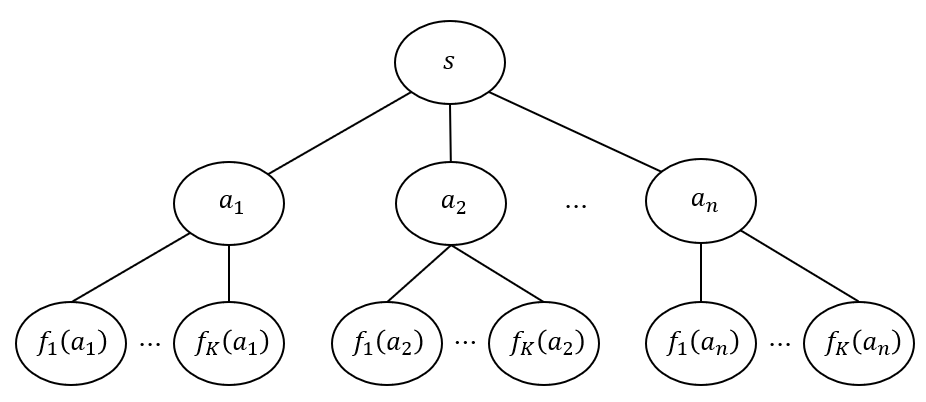
\includegraphics[width=130mm, height=70mm]{Graphics/new_graph.png}
        \caption{Estructura de grafo propuesta}
        \label{fig: graph-struct}
    \end{figure}
\end{center}



\section{Tareas de aprendizaje de m\'aquinas}

El enfoque general para la resoluci\'on del problema es simular el proceso de
construcci\'on de un gr\'afico en un lenguaje de visualizaci\'on.

\begin{itemize}
    \item Seleccionar un atributo del conjunto de datos
    \item Seleccionar secuencialmente las opciones deseadas en la configuraci\'on gr\'afica de la visualizaci\'on: \begin{itemize}
        \item \bf Eje : x, y
        \item \bf Marca : barra, l\'inea, punto
        \item \bf Color : rojo, verde, azul
    \end{itemize}
\end{itemize}

Para generar el gr\'afico el usuario resuelve una serie de problemas de decisi\'on sobre las configuraciones gr\'aficas,
por este motivo dado un lenguaje de visualizaci\'on $\mathcal{C}$ con configuraciones gr\'aficas $C_1, C_2, ..., C_n$
definimos una tarea de aprendizaje de m\'aquinas por cada configuraci\'on $C_i$.

Es importante resaltar que se consideraron dos tipos de configuraciones gr\'aficas: las asociadas
a los atributos (p.e. eje, color, marca) y las asociadas al conjunto de datos (p.e. utilizaci\'on de leyendas y cuadr\'iculas).
La primeras dos tareas propuestas est\'an enfocadas a configuraciones de atributos y la tarea restante se utiliza para
las configuraciones de los conjuntos de datos.

\subsection{Problema de clasificaci\'on de v\'ertices}

Sean un grafo $G = (V,E)$ con $V = V_D \cup V_A \cup V_F$ y $E = E_{DA} \cup E_{AF}$, una configuraci\'on
gr\'afica $C$ y un conjunto $\mathcal{L}$ de etiquetas tal que existe una funci\'on biyectiva $f : \mathcal{L} \to C$.
Dado un conjunto de v\'ertices ${V_D}_l \subset V_D $ los cuales est\'an etiquetados el objetivo es aproximar la funci\'on
$h : V_D \to \mathcal{L}$ para inferir las
etiquetas para el conjunto $V_D \setminus {V_D}_l$ de v\'ertices no etiquetados. 

\subsection{Problema de predicci\'on de aristas}

Para este problema se modific\'o la arquitectura del grafo mostrada por la Figura \ref{fig: graph-struct}
a\~nadiendo el conjunto de v\'ertices $V_C$ el cual representa las posibles opciones de una configuraci\'on $C_i$ y
el conjunto de aristas $E_{AC}$ las cuales representan la utilizaci\'on una opci\'on para codificar un atributo.

\begin{figure}[h!]
    \centering
    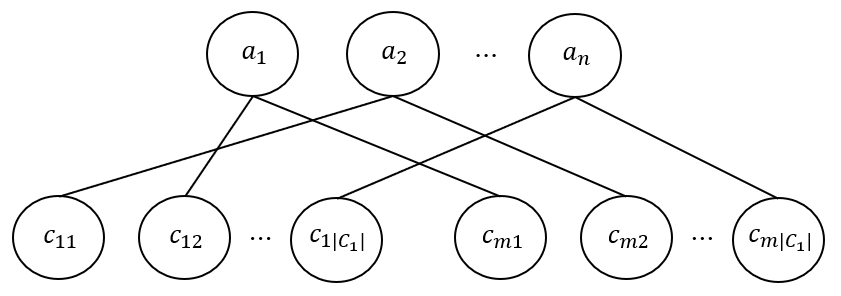
\includegraphics[width=130mm, height=65mm]{Graphics/new_link_pred.png}
    \caption{Estructura de grafo propuesta para el problema de predicci\'on de aristas (Se omiti\'o el resto del grafo por simplicidad).}
    \label{fig: link-pred-graph}
\end{figure}

Sean un grafo $G = (V,E)$ con $V = V_D \cup V_A \cup V_F \cup V_C$ y $E = E_{DA} \cup E_{AF} \cup E_{AC}$,
una configuraci\'on gr\'afica $C$ y $E_{AC}^*$ el conjunto de todas las posibles aristas entre los conjuntos de v\'ertices $V_A$ y $V_C$.
El objetivo es aproximar una funci\'on de probabilidad $p : E_{AC}^* \to [0,1]$ la cual indique la probabilidad de que una arista
entre un elemento $V_A$ y un elemento de $V_C$ pertenezca al grafo.\\\\\\

\subsection{Problema de clasificaci\'on de grafos}

Sean $C$ una configuraci\'on gr\'afica, $\mathcal{L}$ un conjunto de etiquetas y
una funci\'on biyectiva $f : \mathcal{L} \to C$. Dado un conjunto
de grafos etiquetados $\{(G_1, l_1), (G_2, l_2),..., (G_n, l_n)\}$, $l_i \in \mathcal{L} : 1 \leq i \leq n$ 
el objetivo es aproximar una funci\'on $h : \mathbb{G} \to \mathcal{L}$ donde
$\mathbb{G}$ es el espacio de todos los posibles grafos.



\chapter{MLG4Vis}\label{chapter:proposal}

En la actualidad los analistas de datos realizan su trabajo
sobre conjuntos de datos de gran tama\~no y dimensi\'on por lo que
necesitan de herramientas computacionales que apoyen y faciliten
su trabajo en la toma de decisiones, sobre todo cuando tratan con una
cantidad de informaci\'on considerable.

En esta secci\'on se describe un prototipo de sistema de recomendaci\'on de
configuraciones gr\'aficas basado en el marco de trabajo definido
en el Cap\'itulo \ref{chapter:ml-on-graphs}, con el objetivo de que pueda ser utilizado
por plataformas de an\'alisis de datos, sea dentro de un an\'alisis manual o 
automatizado.\\

\section{Concepci\'on y dise\~no del sistema}

\begin{figure}[h!]
    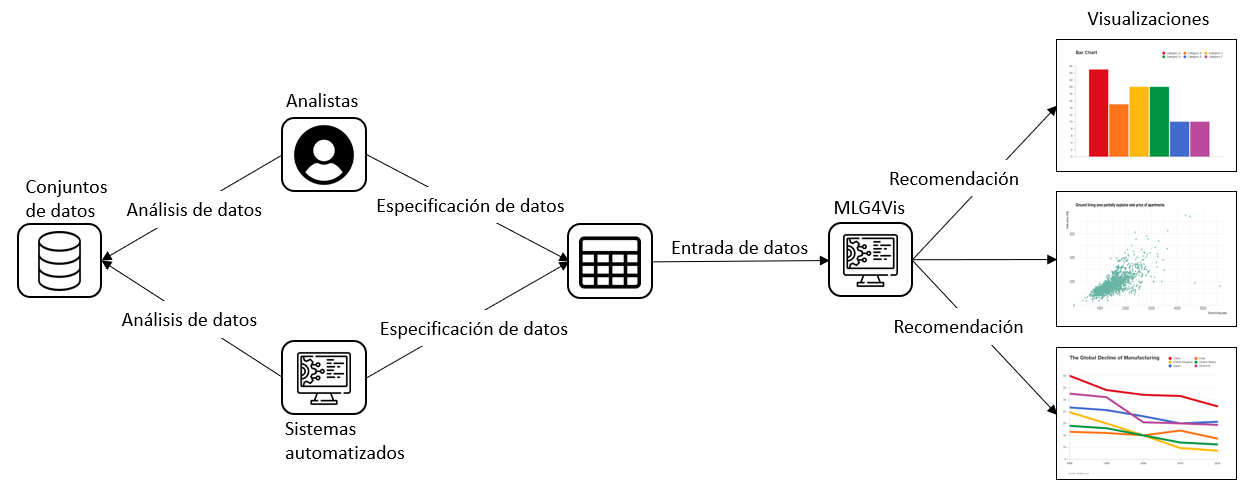
\includegraphics[width=\linewidth]{Graphics/mlg4vis.png}
    \caption{Utilizaci\'on de MLG4Vis en el an\'alisis de datos}
    \label{fig: mlg4vis}
\end{figure}


\textit{Machine Learning on Graphs For Visualization} (GML4Vis) se concibe como un
sistema el cual pueda ser utilizado dentro de plataformas de an\'alisis de datos. Estas plataformas
deben permitir una especificaci\'on parcial de las visualizaciones, pudiendo el
usuario definir la informaci\'on a ser visualizada u obtener esta mediante sistemas
automatizados como LETO (Figura \ref{fig: mlg4vis}).

GML4Vis est\'a dividido en 4 m\'odulos interrelacionados que
constituyen la implementaci\'on del enfoque propuesto en el Cap\'itulo \ref{chapter:ml-on-graphs}.
Cada m\'odulo
tiene una responsabilidad espec\'ifica mediante la definici\'on de datos
de entrada y salida que definen la intercomunicaci\'on con el resto de los
m\'odulos. La Figura \ref{fig: mlg4vis-arch} permite tener una
visi\'on de la arquitectura del sistema.

\begin{figure}[h!]
    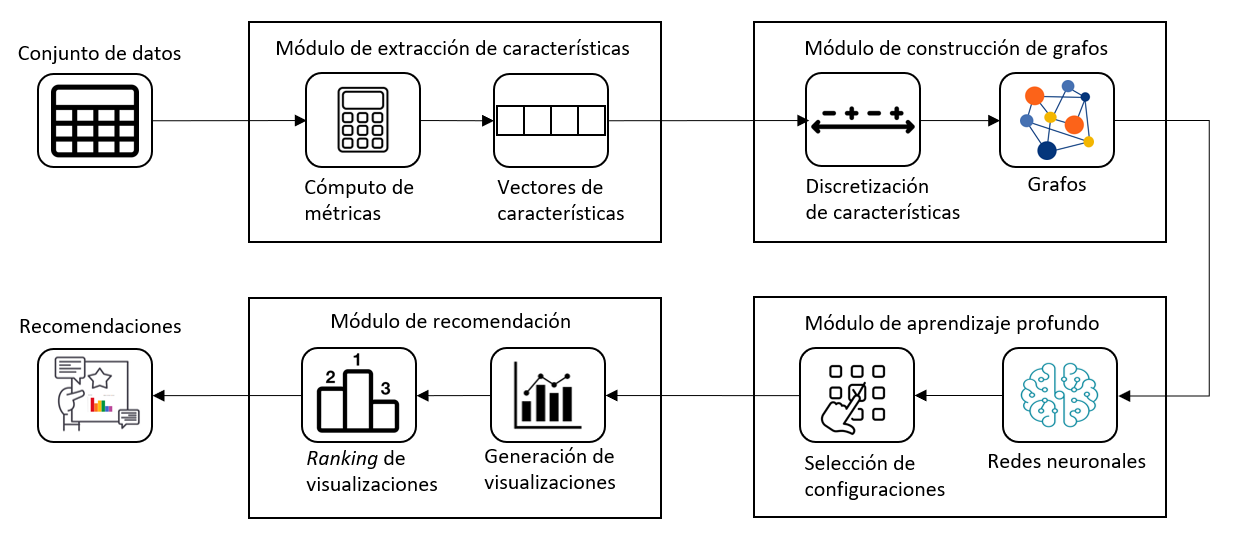
\includegraphics[width=\linewidth]{Graphics/pipeline.png}
    \caption{Arquitectura de GML4Vis}
    \label{fig: mlg4vis-arch}
\end{figure}

Como se puede apreciar en la Figura \ref{fig: mlg4vis-arch} los
4 m\'odulos est\'an dispuestos de forma secuencial modelando
la transformaci\'on de un conjunto de datos en recomendaciones.

\begin{itemize}
    \item La entrada del sistema la constituye un conjunto de datos estructurados.
    \item El \textbf{M\'odulo de extracci\'on de caracter\'isticas} computa una serie
    de m\'etricas que permiten describir el conjunto de datos como un conjunto de vectores de caracter\'isticas.
    \item El \textbf{M\'odulo de construcci\'on de grafos} realiza un proceso de discretizaci\'on
    sobre las caracter\'isticas continuas de los vectores y procede a construir los grafos propuestos
    en el Cap\'itulo \ref{chapter:ml-on-graphs}.
    \item El \textbf{M\'odulo de aprendizaje profundo} este m\'odulo implementa los modelos
    de redes neuronales que seleccionan las configuraciones gr\'aficas mediante la resoluci\'on
    de las tareas propuestas en el Cap\'itulo \ref{chapter:ml-on-graphs}.
    \item El \textbf{M\'odulo de recomendaci\'on} se encarga de construir las visualizaciones
    utilizando las configuraciones seleccionadas por las redes neuronales y realiza un \textit{ranking}
    de las visualizaciones.
    \item El \textit{ranking} de visualizaciones obtenido se retorna como salida del sistema en forma de
    recomendaciones.
\end{itemize}

En las secciones a continuaci\'on se expone de forma general el funcionamiento de los distintos m\'odulos
del sistema y las principales consideraciones tomadas durante su dise\~no.

\subsection{M\'odulo de extraci\'on de caracter\'isticas}

Este m\'odulo se encarga de transformar el conjunto de datos de entrada a un
espacio com\'un de vectores de $K$ dimensiones mediante el c\'omputo de m\'etricas. 

Antes de realizar el c\'alculo de las m\'etricas se realizan dos pasos de preprocesamiento.
Primeramente se realiza (de ser necesario) una inferencia del tipo de los atributos del conjunto de datos ya que existen
varios formatos de almacenamiento de datos (p.e. valores separados por comas) que no almacenan los metadatos
respectivos al dominio de los atributos. Luego se aborda un problema com\'un dentro del an\'alisis de datos que
es la existencia de datos faltantes \cite{schafer2002missing}. Este problema ha sido extensamente estudiado en la
rama de la Estad\'istica debido a que puede comprometer la calidad de las mediciones estad\'isticas obtenidas, para
resolver este problema se utilizaron t\'ecnicas de imputaci\'on de datos \cite{jadhav2019comparison}.

Terminado el preprocesamiento se procede a realizar el c\'alculo de una serie de medidas. La mayor\'ia
de estas medidas provienen del campo de la Estad\'istica y fueron seleccionadas de acuerdo a su robustez
ante la diferencia de magnitudes que pueden existir en los distintos conjuntos de datos.

\subsection{M\'odulo de construcci\'on de grafos}

Previo a la construcci\'on del grafo se realiza un proceso
de discretizaci\'on de las componentes de los vectores, con el de objetivo reducir
la cantidad de v\'ertices del grafo que surgen como la representaci\'on de valores en un dominio continuo.
Cada componente es discretizada mediante la creaci\'on de intervalos que particionan el
rango de valores que puede tomar. Para este proceso
se utiliz\'o el algoritmo MDLP \cite{fayyad1993multi} el cual puede
inferir la cantidad de intervalos en que deben ser particionados los valores
bas\'andose en la distribuci\'on de los datos.

Luego se procede a construir los grafos de acuerdo a las estructuras propuestas en el Cap\'itulo \ref{chapter:ml-on-graphs}.

\subsection{M\'odulo de aprendizaje profundo}

Luego de obtenidos los grafos que modelan los conjuntos de datos se procede
a dise\~nar modelos que resuelvan las tareas de aprendizaje de m\'aquinas definidas en el Cap\'itulo \ref{chapter:ml-on-graphs}.

En este trabajo se utilizan modelos basados en \textit{Graph Representation Learning} (Secci\'on \ref{section:theoretical-framework}) debido
a dos motivos principales:

\begin{itemize}
    \item Los enfoques tradicionales al aprendizaje de m\'aquinas sobre grafos son
    basados principalmente en el c\'alculo de m\'etricas o propiedades del grafo. Esto
    hace que los resultados de dichos m\'etodos sean muy sensibles a datos no observados
    durante el entrenamiento. Debido a que los analistas trabajan con nuevos conjuntos de datos
    de forma constante es importante utilizar modelos que puedan presentar buenos resultados con datos no observados.
    \item Los enfoques basados en GRL son muy parecidos
    a los utilizados en el aprendizaje de m\'aquinas tradicional, lo que coincide con el
    \'area de investigaci\'on de los tutores de este trabajo.
\end{itemize}

Dentro de GRL existen m\'ultiples algoritmos para solucionar las tareas propuestas [\cite*{hamilton2017representation}, \cite*{chami2022machine},  \cite*{cai2018comprehensive}, \cite*{nickel2015review}], por lo que a continuaci\'on se presentan
los criterios utilizados en la selecci\'on de algoritmos para este escenario.

\begin{itemize}
    \item El algoritmo debe de poder utilizarse sobre grafos heterog\'eneos con v\'ertices y aristas de distintos tipos.
    \item El algoritmo debe ser robusto ante la presencia de datos no observados.
    \item El algoritmo debe de ser eficiente computacionalmente.
\end{itemize}

El algoritmo seleccionado fue Heterogeneous GraphSAGE (HinSAGE) \cite{hinsage}, una generalizaci\'on del
algoritmo GraphSAGE \cite{hamilton2017inductive} para grafos heterog\'eneos. HinSAGE es un algoritmo \textit{inductivo}
para solucionar el problema de \textit{graph embedding} (Cap\'itulo \ref{section:theoretical-framework}) que ha sido
utilizado en m\'ultiples problemas de aprendizaje de m\'aquinas sobre grafos en los \'ultimos a\~nos
[ \cite*{racchi2021fraud}, \cite*{yacoumatos2021trialgraph}, \cite*{cho2022heterogeneous}, \cite*{van2022inductive}].
Utilizando redes neuronales aprende una funci\'on que
genera \textit{embeddings} de los v\'ertices del grafo y este enfoque inductivo le permite transformar v\'ertices
no observados durante el entrenamiento. En cuanto a la eficiencia al estar
basado en redes neuronales es eficiente computacionalmente pero costoso espacialmente.

% A partir de la investigaci\'on se desarrollaron dos modelos distintos:

% \begin{itemize}
%     \item El primer modelo est\'a enfocado a la soluci\'on de las tareas de clasificaci\'on de v\'ertices y clasificaci\'on de grafos.
%     Este modelo utiliza la estrategia \textit{One vs All} para las tareas de clasificaci\'on multiclase, esta se
%     basa en construir un clasificador por cada clase y entrenarlo en un problema de clasificaci\'on binario de \textit{pertenece o no a la clase}.
%     Luego para seleccionar una clase todos los modelos entrenados emiten un voto y la clase m\'as votada es la elegida como correcta.
%     La utilizaci\'on de este enfoque en lugar de utilizar una \'unica red neuronal se debe a la necesidad de obtener una medida de la ``confianza''
%     del clasificador en su decisi\'on para poder realizar un \textit{r\'anking}. Esta confianza puede ser modelada como la cantidad de votos
%     recibidos entre la cantidad de votos totales.
%     \item El segundo modelo est\'a enfocado en la soluci\'on de la tarea de predicci\'on de aristas, dado que el objetivo de este problema es obtener una probabilidad
%     para cada arista se pudo utilizar una \'unica red neuronal.
% \end{itemize}

La estructura neuronal propuesta para 

\subsection{M\'odulo de recomendaci\'on}

Utilizando las distribuciones de probabilidades generadas por las redes neuronales es posible realizar
recomendaciones modelando la selecci\'on de opciones como un conjunto de sucesos independientes.

Consid\'erese una lista de configuraciones visuales $C_1, C_2, ..., C_n$ y las distribuciones de probabilidades 
$p_1, p_2, ..., p_n$ computadas por los modelos GRL tal que $p_i$ es la distribuci\'on de probabilidades
de la configuraci\'on $C_i$.
La probabilidad de una visualizaci\'on $g = <c_1, c_2, ..., c_n> \in C_1 \times C_2 \times ... \times C_n$
se define como $p(g) = p_1(c_1) \cdot p_2(c_2) \cdot ... \cdot p_n(c_n)$.
Con esta definici\'on se garantiza que las visualizaciones en los primeros puestos del \textit{ranking} 
est\'en construidas utilizando solamente opciones de alta probabilidad 
de ocurrencia ya que $\exists \; c_i : p(c_i) \to 0 \implies p(g) \to 0$.


\section{Corpus}

Para poder implementar este sistema, y en general
para todos los algoritmos de aprendizaje supervisado, se hace necesario contar con datos previamente clasificados.
En el contexto de la generaci\'on de configuraciones visuales esos datos ser\'ian conjuntos
de datos con su respectiva visualizaci\'on asociada. Para extraer las configuraciones gr\'aficas 
estas visualizaciones deben de estar especificadas en lenguajes de visualizaci\'on de datos u otros lenguajes
de intercambio de datos como JSON \cite{pezoa2016foundations}.

A pesar de la relevancia de las funciones de recomendaci\'on dentro
de las herramientas de an\'alisis de datos el progreso en esta l\'inea
de investigaci\'on es lastrado por la inexistencia de grandes corpus p\'ublicos.
Repositorios como WordNet \cite{wordnet1998} y IMDB Reviews \cite{maas-EtAl:2011:ACL-HLT2011} han jugado un papel importante en el desarrollo actual
del procesamiento de lenguaje natural, sin embargo, no existen repositorios similares para
los problemas enmarcados en la visualizaci\'on autom\'atica de datos.

Al momento de realizarse la presente investigaci\'on los corpus existentes
han sido creados durante el desarrollo de sistemas basados en el aprendizaje de m\'aquinas (Cap\'itulo \ref{chapter:state-of-the-art}).
Data2Vis cre\'o un corpus mediante la utilizaci\'on del sistema basado en reglas Voyager. Draco-Learn y DeepEye encargaron
la construcci\'on del corpus a un conjunto de expertos en visualizaci\'on de datos. Finalmente VizML construy\'o el primer corpus
de gran tama\~no mediante la recolecci\'on de visualizaciones publicadas en la plataforma Plotly \cite{plotly}. Debido a la gran cantidad
de datos necesitada para el entrenamiento y validaci\'on de modelos de redes neuronales se opt\'o por utilizar el corpus de Plotly para el desarrollo de
este trabajo. 

